\documentclass[12pt]{article}
\usepackage{setspace, graphicx, fullpage, amssymb, amsmath, epsfig, natbib, array, multirow, hyperref}
\usepackage{amsfonts, bm} 
\usepackage{dcolumn}
\usepackage{subfigure, float} 
\usepackage[margin=1in]{geometry} 
\usepackage{verbatim}
\usepackage{url}
\usepackage{enumerate}
\newcolumntype{d}[1]{D{.}{.}{#1}} 

\begin{document}
	
\begin{center}
	\Large 22 February 2017, cont.
\end{center}
	
\section{Tables and Figures, cont.}
	
\subsection{House lm Descriptive Statistics}

% latex table generated in R 3.3.2 by xtable 1.8-2 package
% Mon Feb 20 20:13:00 2017
\begin{table}[ht]
	\centering
	\begin{tabular}{rrrr}
		\hline
		congress & party calls & noncalls & gray votes \\ 
		\hline
		93 & 504 & 535 &   3 \\ 
		94 & 601 & 599 &   7 \\ 
		95 & 660 & 806 &   4 \\ 
		96 & 631 & 596 &   1 \\ 
		97 & 425 & 289 &  63 \\ 
		98 & 542 & 298 &  15 \\ 
		99 & 523 & 318 &   2 \\ 
		100 & 559 & 289 &   4 \\ 
		101 & 496 & 318 &   2 \\ 
		102 & 569 & 251 &  24 \\ 
		103 & 754 & 278 &   6 \\ 
		104 & 857 & 392 &   0 \\ 
		105 & 592 & 481 &   2 \\ 
		106 & 768 & 226 &  79 \\ 
		107 & 640 & 169 &   1 \\ 
		108 & 627 & 251 & 102 \\ 
		109 & 659 & 288 &  91 \\ 
		110 & 1087 & 316 & 147 \\ 
		111 & 787 & 340 &  84 \\ 
		112 & 1272 & 173 &  80 \\
		\hline
		Total: & 13553 & 7213 & 717 \\
		Mean: & 677.7 & 360.7 & 35.9 \\
		sd: & 204.4 & 162.7 & 45.4 \\
		\hline
	\end{tabular}
\end{table}

% latex table generated in R 3.3.2 by xtable 1.8-2 package
% Mon Feb 20 20:21:26 2017
\begin{table}[ht]
	\centering
	\begin{tabular}{rrrr}
		\hline
		& party call & noncall & gray \\ 
		\hline
		lopsided & 4245 & 6123 & 686 \\ 
		close & 9308 & 1090 &  31 \\ 
		\hline
	\end{tabular}
\end{table}

% Table created by stargazer v.5.2 by Marek Hlavac, Harvard University. E-mail: hlavac at fas.harvard.edu
% Date and time: Mon, Feb 20, 2017 - 20:49:00
\begin{table}[!htbp] \centering 
	\caption{Responsiveness Statistics} 
	\label{} 
	\begin{tabular}{@{\extracolsep{5pt}}lccccc} 
		\\[-1.8ex]\hline 
		\hline \\[-1.8ex] 
		Statistic & \multicolumn{1}{c}{N} & \multicolumn{1}{c}{Mean} & \multicolumn{1}{c}{St. Dev.} & \multicolumn{1}{c}{Min} & \multicolumn{1}{c}{Max} \\ 
		\hline \\[-1.8ex] 
		Democrats: & & & & & \\
		\hline
		party free ideal point & 4,749 & $-$0.545 & 0.809 & $-$4.076 & 4.317 \\ 
		pirate100 & 4,749 & 86.299 & 12.111 & 8.021 & 100.000 \\ 
		pfrate100 & 4,746 & 86.996 & 7.214 & 0.000 & 100.000 \\ 
		ideological extremism & 4,749 & 0.545 & 0.809 & $-$4.317 & 4.076 \\ 
		\hline
		Republicans: & & & & & \\
		\hline
		party free ideal point & 3,801 & 0.673 & 0.786 & $-$2.473 & 9.347 \\ 
		pirate100 & 3,801 & 85.198 & 10.609 & 31.276 & 100.000 \\ 
		pfrate100 & 3,798 & 86.904 & 7.858 & 28.302 & 100.000 \\ 
		ideological extremism & 3,801 & 0.673 & 0.786 & $-$2.473 & 9.347 \\
		\hline
		Majority Party: & & & & & \\
		\hline
		party free ideal point & 4,905 & $-$0.152 & 0.958 & $-$4.076 & 9.347 \\ 
		pirate100 & 4,905 & 87.612 & 11.446 & 8.021 & 100.000 \\ 
		pfrate100 & 4,902 & 87.078 & 7.587 & 0.000 & 100.000 \\ 
		ideological extremism & 4,905 & 0.526 & 0.814 & $-$4.317 & 9.347 \\ 
		\hline
		Minority Party: & & & & & \\
		\hline
		party free ideal point & 3,645 & 0.197 & 1.027 & $-$3.524 & 4.084 \\ 
		pirate100 & 3,645 & 83.384 & 11.073 & 20.077 & 100.000 \\ 
		pfrate100 & 3,642 & 86.791 & 7.395 & 38.889 & 100.000 \\ 
		ideological extremism & 3,645 & 0.705 & 0.773 & $-$1.756 & 4.084 \\ 
		\hline \\[-1.8ex] 
	\end{tabular} 
\end{table} 

\pagebreak

\subsection{House lm Models}


\begin{table}[!htb]
	\begin{center}
		\caption{Bivariate DV/IV Regressions}
		\begin{tabular}{l c c c c }
			\hline
			& Democrats & Democrats & Republican & Republican \\
			\hline
			pfrate100              & $0.71^{***}$  &               & $0.26^{***}$  &               \\
			& $(0.02)$      &               & $(0.02)$      &               \\
			ideological extremism &               & $9.88^{***}$  &               & $4.67^{***}$  \\
			&               & $(0.16)$      &               & $(0.21)$      \\
			(Intercept)            & $24.69^{***}$ & $80.91^{***}$ & $62.37^{***}$ & $82.05^{***}$ \\
			& $(1.93)$      & $(0.16)$      & $(1.87)$      & $(0.21)$      \\
			\hline
			R$^2$                  & 0.18          & 0.44          & 0.04          & 0.12          \\
			Adj. R$^2$             & 0.18          & 0.44          & 0.04          & 0.12          \\
			Num. obs.              & 4746          & 4749          & 3798          & 3801          \\
			RMSE                   & 10.98         & 9.10          & 10.40         & 9.95          \\
			\hline
			\multicolumn{5}{l}{\scriptsize{$^{***}p<0.001$, $^{**}p<0.01$, $^*p<0.05$}}
		\end{tabular}
	\end{center}
\end{table}

\begin{table}[!htb]
	\begin{center}
		\caption{Multivariate DV/IV Regressions}
		\begin{tabular}{l c c c c }
			\hline
			& Democrats & Republicans & Majority & Minority \\
			\hline
			pfrate100              & $0.690^{***}$  & $0.434^{***}$  & $0.593^{***}$  & $0.650^{***}$  \\
			& $(0.015)$      & $(0.020)$      & $(0.015)$      & $(0.020)$      \\
			ideological extremism & $9.791^{***}$  & $5.940^{***}$  & $8.047^{***}$  & $9.666^{***}$  \\
			& $(0.136)$      & $(0.203)$      & $(0.142)$      & $(0.193)$      \\
			(Intercept)            & $20.907^{***}$ & $43.427^{***}$ & $31.709^{***}$ & $20.154^{***}$ \\
			& $(1.337)$      & $(1.812)$      & $(1.328)$      & $(1.810)$      \\
			\hline
			R$^2$                  & 0.606          & 0.216          & 0.503          & 0.428          \\
			Adj. R$^2$             & 0.606          & 0.215          & 0.503          & 0.428          \\
			Num. obs.              & 4746           & 3798           & 4902           & 3642           \\
			RMSE                   & 7.603          & 9.394          & 8.067          & 8.370          \\
			\hline
			\multicolumn{5}{l}{\scriptsize{$^{***}p<0.001$, $^{**}p<0.01$, $^*p<0.05$}}
		\end{tabular}
	\end{center}
\end{table}

\begin{figure}[ht]
	\caption{Main DV and Ideological Extremism - Southern and Other House Democrats}
	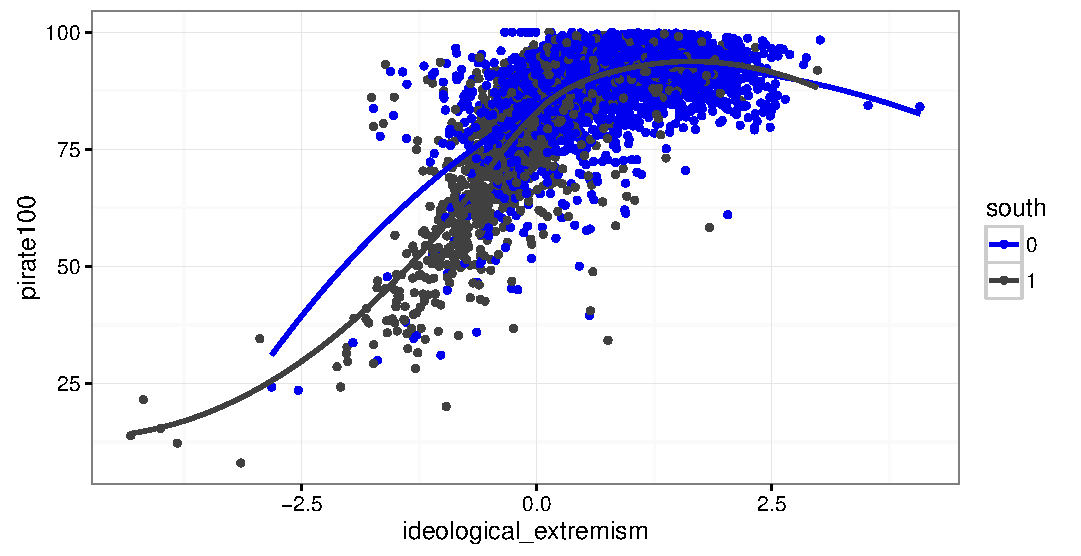
\includegraphics[width = \textwidth]{C:/Users/Ethan/Documents/GitHub/partycalls/plots/house_lm_dem_iv-dv_south.pdf}
\end{figure}

\begin{figure}[ht]
	\caption{Main DV and Ideological Extremism - Majority and Minority House Democrats}
	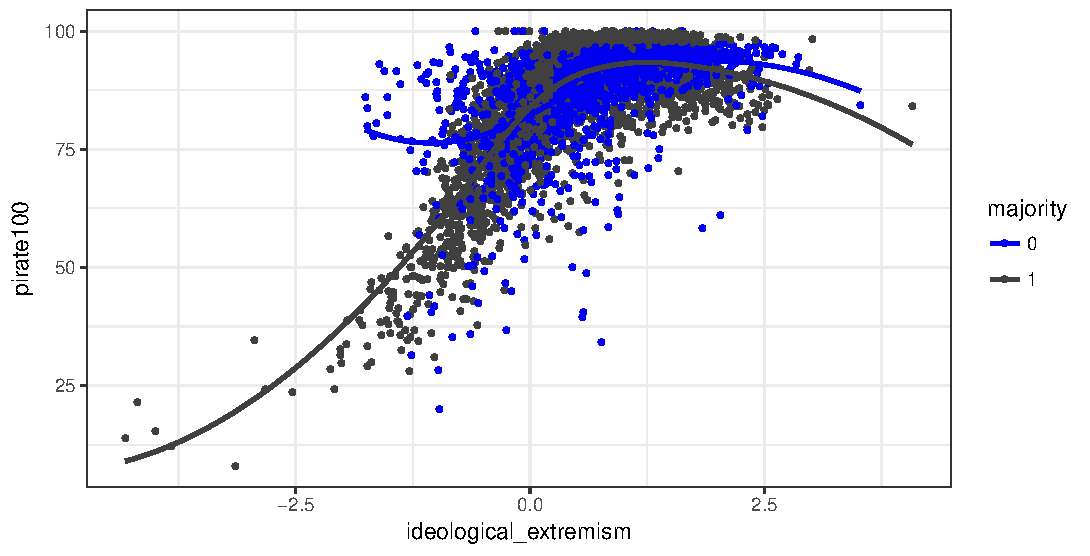
\includegraphics[width = \textwidth]{C:/Users/Ethan/Documents/GitHub/partycalls/plots/house_lm_dem_iv-dv_majority.pdf}
\end{figure}

\begin{figure}[ht]
	\caption{Main DV and Ideological Extremism - Southern and Other House Republicans}
	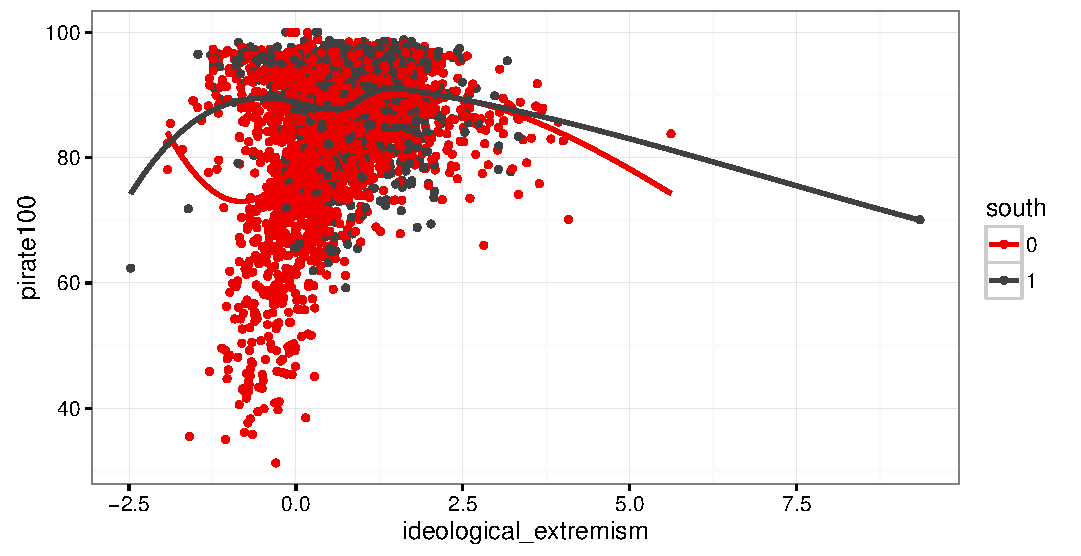
\includegraphics[width = \textwidth]{C:/Users/Ethan/Documents/GitHub/partycalls/plots/house_lm_rep_iv-dv_south.pdf}
\end{figure}

\begin{figure}[ht]
	\caption{Main DV and Ideological Extremism - Majority and Minority House Republicans}
	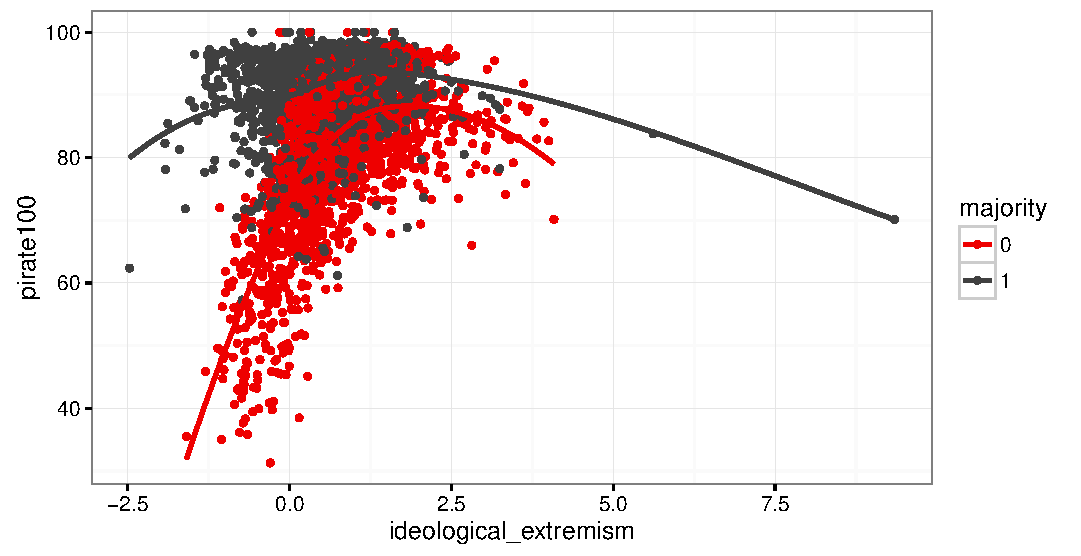
\includegraphics[width = \textwidth]{C:/Users/Ethan/Documents/GitHub/partycalls/plots/house_lm_rep_iv-dv_majority.pdf}
\end{figure}

\begin{figure}[ht]
	\caption{IV/IV Plot - Southern and Other House Democrats}
	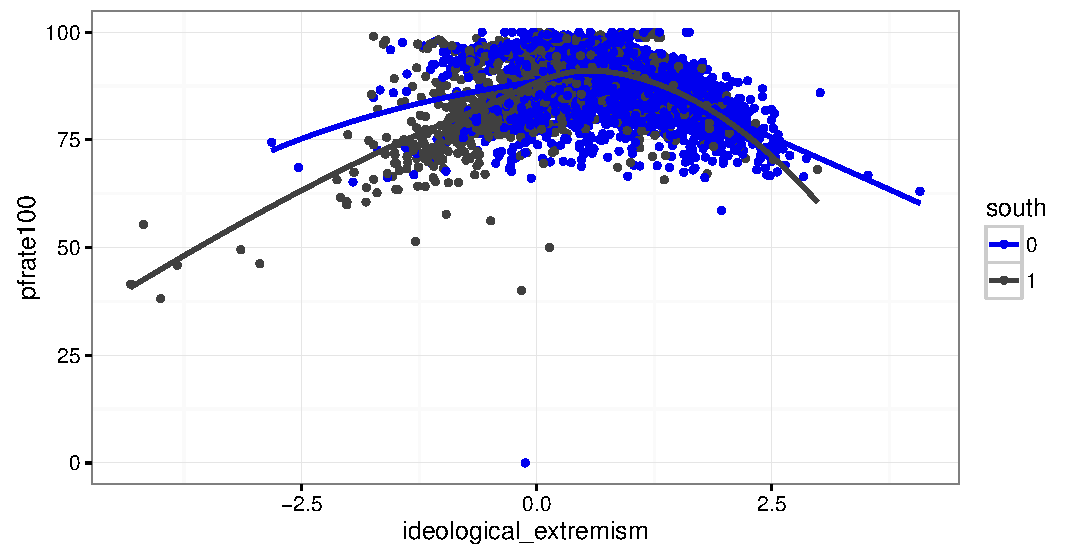
\includegraphics[width = \textwidth]{C:/Users/Ethan/Documents/GitHub/partycalls/plots/house_lm_dem_iv-iv_south.pdf}
\end{figure}

\begin{figure}[ht]
	\caption{IV/IV Plot - Majority and Minority House Democrats}
	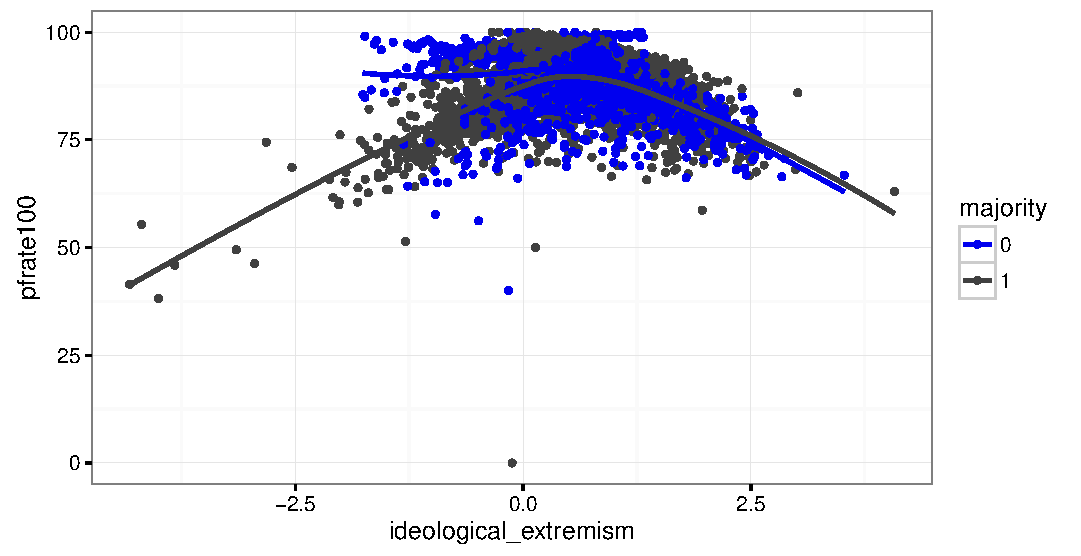
\includegraphics[width = \textwidth]{C:/Users/Ethan/Documents/GitHub/partycalls/plots/house_lm_dem_iv-iv_majority.pdf}
\end{figure}

\begin{figure}[ht]
	\caption{IV/IV Plot - Southern and Other House Republicans}
	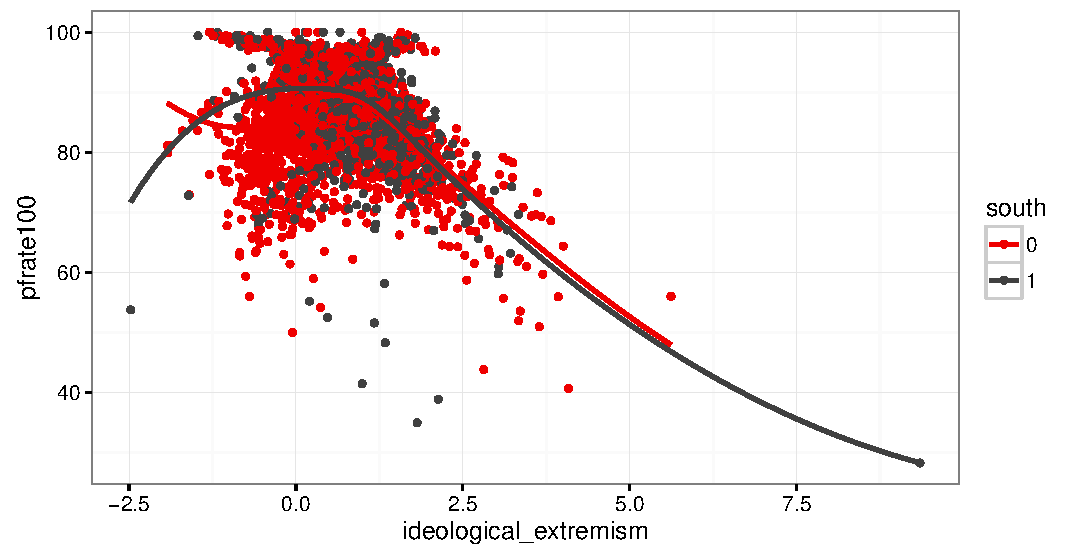
\includegraphics[width = \textwidth]{C:/Users/Ethan/Documents/GitHub/partycalls/plots/house_lm_rep_iv-iv_south.pdf}
\end{figure}

\begin{figure}[ht]
	\caption{IV/IV Plot - Majority and Minority House Republicans}
	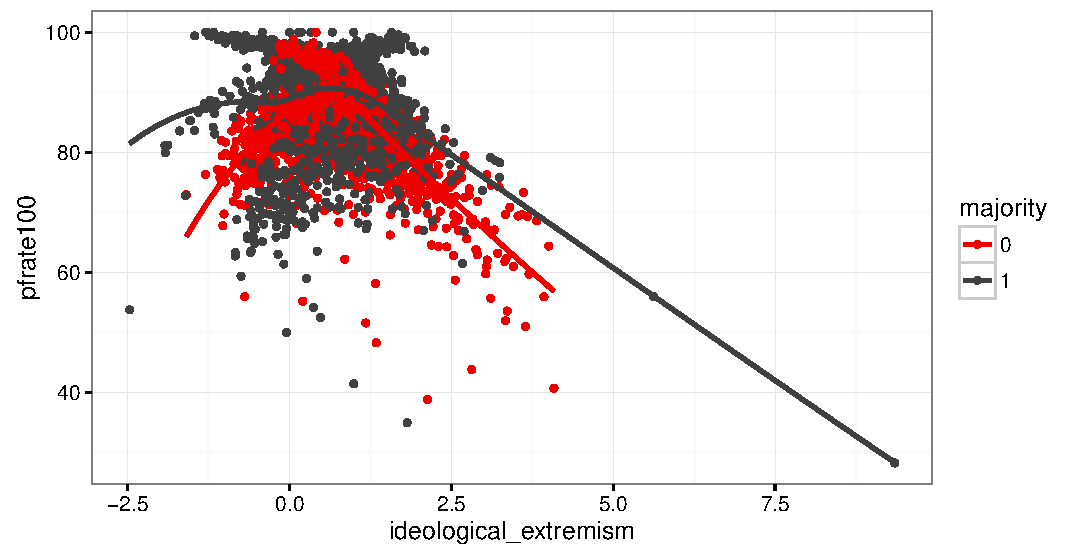
\includegraphics[width = \textwidth]{C:/Users/Ethan/Documents/GitHub/partycalls/plots/house_lm_rep_iv-iv_majority.pdf}
\end{figure}

\begin{table}[ht]
	\begin{center}
		\caption{Full Regression Tables}
		\begin{tabular}{l c c c c }
			\hline
			& Democrats & Republicans & Majority & Minority \\
			\hline
			(Intercept)            & $24.00^{***}$ & $53.05^{***}$ & $36.42^{***}$ & $17.69^{***}$ \\
			& $(1.58)$      & $(2.21)$      & $(1.49)$      & $(2.05)$      \\
			ideological\_extremism & $8.34^{***}$  & $5.84^{***}$  & $6.64^{***}$  & $8.73^{***}$  \\
			& $(0.17)$      & $(0.21)$      & $(0.16)$      & $(0.20)$      \\
			pfrate100              & $0.64^{***}$  & $0.41^{***}$  & $0.52^{***}$  & $0.63^{***}$  \\
			& $(0.02)$      & $(0.02)$      & $(0.01)$      & $(0.02)$      \\
			pres\_votepct          & $0.09^{***}$  & $-0.09^{***}$ & $0.20^{***}$  & $0.17^{***}$  \\
			& $(0.01)$      & $(0.02)$      & $(0.01)$      & $(0.02)$      \\
			south                  & $-2.43^{***}$ & $3.63^{***}$  & $-1.65^{***}$ & $-0.36$       \\
			& $(0.28)$      & $(0.34)$      & $(0.25)$      & $(0.31)$      \\
			votepct                & $-0.04^{***}$ & $-0.00$       & $-0.09^{***}$ & $-0.07^{***}$ \\
			& $(0.01)$      & $(0.01)$      & $(0.01)$      & $(0.01)$      \\
			female                 & $0.53$        & $-0.08$       & $-0.13$       & $2.12^{***}$  \\
			& $(0.35)$      & $(0.58)$      & $(0.40)$      & $(0.44)$      \\
			afam                   & $-0.52$       & $5.02$        & $-3.04^{***}$ & $3.23^{***}$  \\
			& $(0.44)$      & $(2.98)$      & $(0.53)$      & $(0.61)$      \\
			latino                 & $1.73^{***}$  & $2.42^{*}$    & $2.83^{***}$  & $3.01^{***}$  \\
			& $(0.51)$      & $(1.16)$      & $(0.63)$      & $(0.70)$      \\
			seniority              & $0.05$        & $-0.33^{***}$ & $0.02$        & $0.01$        \\
			& $(0.03)$      & $(0.05)$      & $(0.03)$      & $(0.04)$      \\
			freshman               & $-0.07$       & $1.01^{*}$    & $0.28$        & $-0.40$       \\
			& $(0.36)$      & $(0.46)$      & $(0.35)$      & $(0.44)$      \\
			bestgrosswart          & $-0.04^{*}$   & $-0.24^{***}$ & $-0.17^{***}$ & $-0.16^{***}$ \\
			& $(0.02)$      & $(0.03)$      & $(0.02)$      & $(0.02)$      \\
			leader                 & $1.96^{**}$   & $2.79^{***}$  & $2.62^{***}$  & $1.78^{**}$   \\
			& $(0.60)$      & $(0.76)$      & $(0.65)$      & $(0.65)$      \\
			power                  & $1.82^{***}$  & $2.94^{***}$  & $3.02^{***}$  & $1.05^{**}$   \\
			& $(0.28)$      & $(0.37)$      & $(0.27)$      & $(0.36)$      \\
			chair                  & $2.46^{***}$  & $9.57^{***}$  & $1.85^{***}$  & $-7.98$       \\
			& $(0.50)$      & $(0.80)$      & $(0.44)$      & $(4.63)$      \\
			\hline
			R$^2$                  & 0.63          & 0.30          & 0.57          & 0.48          \\
			Adj. R$^2$             & 0.63          & 0.30          & 0.56          & 0.48          \\
			Num. obs.              & 4746          & 3798          & 4902          & 3642          \\
			RMSE                   & 7.36          & 8.88          & 7.55          & 8.01          \\
			\hline
			\multicolumn{5}{l}{\scriptsize{$^{***}p<0.001$, $^{**}p<0.01$, $^*p<0.05$}}
		\end{tabular}
	\end{center}
\end{table}

\begin{figure}[h]
	\centering
	\caption{House lm Coefficient Plot}
	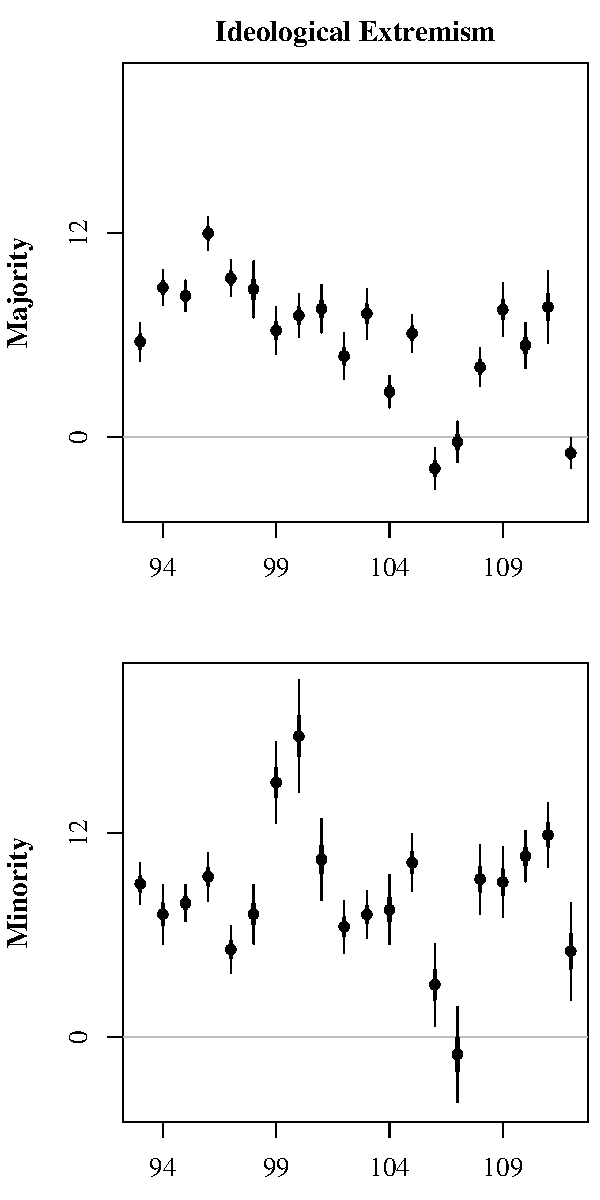
\includegraphics[width = 10cm]{C:/Users/Ethan/Documents/GitHub/partycalls/plots/who-heeds-figure2-replication_lm.pdf}
\end{figure}
























\end{document}